% Encoder architecture of the local-sla-15yr AnemoiModelEncProcDec.
%
%   page 1  the encoder wire diagram, drawn entirely in symbols
%   page 2  the notation table, with the values read out of the checkpoint
%
% Build:  make            (regenerates dims.tex / symbols_table.tex first)
%         latexmk -pdf network_diagram.tex
%
% To drop the figure alone into a paper, % ---------------------------------------------------------------------------
% Encoder of AnemoiModelEncProcDec (GraphTransformerForwardMapper), drawn at the
% block level of "Attention Is All You Need" Fig. 1, with every wire annotated
% by its array shape.
%
% The tikzpicture only -- \input it into a document whose preamble loads
% notation.tex and the tikz libraries listed in network_diagram.tex.
%
% Layout: three lanes flowing left to right --
%   DATA   (top)     x-space nodes:  psi -> Linear -> LayerNorm -> key, value
%   EDGE   (middle)  encoder edges:  a_e -> Linear -> eps
%   LATENT (bottom)  z-space nodes:  a_z -> Linear -> LayerNorm -> query, self
% converging at the graph attention block, after which the latent stream
% continues alone along the middle line.
%
% Every node is placed off the \row*/\col* registers below, so the figure is
% reflowed by editing numbers in one place rather than by moving nodes.
% ---------------------------------------------------------------------------

% --- lane (row) positions ---------------------------------------------------
\def\rowdata{0}          % data-space lane
\def\rowedge{-6.0}       % edge lane; also the latent stream after attention
\def\rowlat{-12.0}        % latent-space lane
\def\rowbypass{4.2}      % raw psi running over the top to the decoder
\def\rowconn{-9.0}       % graph connectivity entering the attention block
\def\rowselfskip{-16.0}  % self branch routed under the attention block
\def\rowdstskip{-18.6}   % pre-norm latent skip routed under everything
\def\rowffskip{-3.0}     % skip around the feed forward

% --- column positions -------------------------------------------------------
\def\colA{0}        % inputs
\def\colcat{4.8}    % concatenation
\def\colB{7.7}      % embedding Linear
\def\colC{11.4}     % LayerNorm
\def\colD{15.4}     % q / k / v / edge projections
\def\colsplit{13.4} % where a LayerNorm output branches in two
\def\colE{21.6}     % graph attention
\def\colF{26.6}     % residual 1
\def\colG{29.4}     % projection
\def\colH{32.6}     % residual 2
\def\colI{35.6}     % LayerNorm + feed forward
\def\colJ{38.6}     % residual 3
\def\colK{40.8}     % output

\def\stack{1.15}    % vertical offset of paired sub-boxes

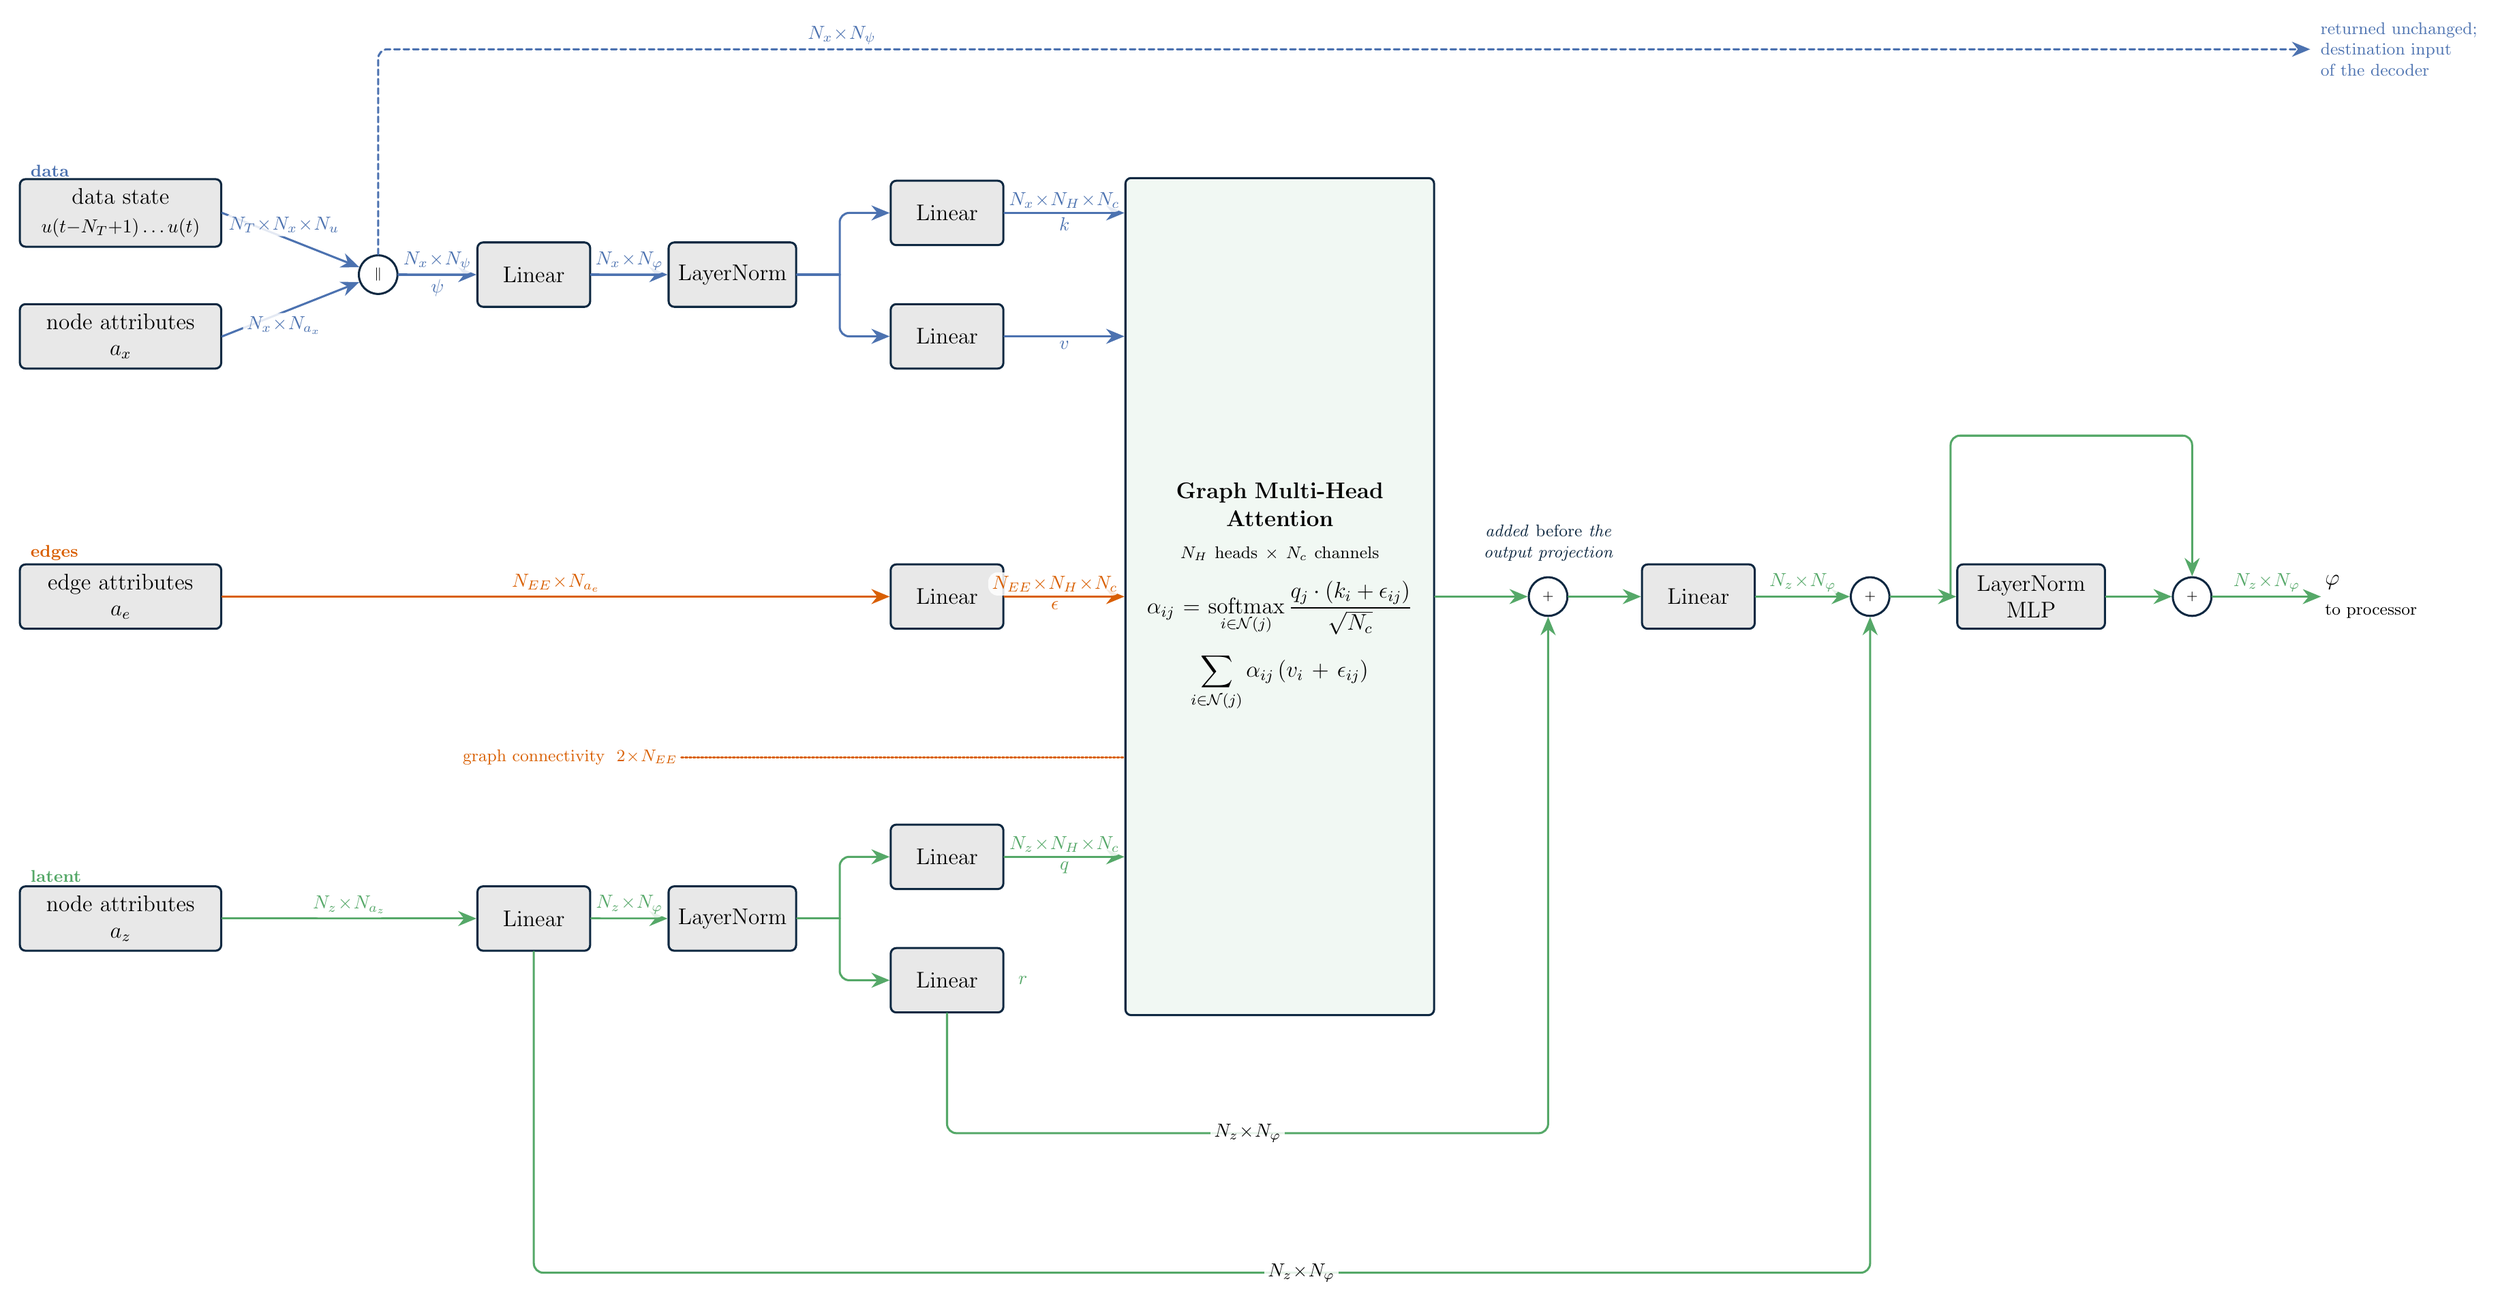
\begin{tikzpicture}[
  x=1cm, y=1cm, font=\large,
  blk/.style     = {rounded corners=3pt, draw=trapline, fill=trapfill,
                    line width=1.1pt, align=center, inner sep=5pt,
                    minimum height=1.2cm, minimum width=2.1cm},
  attnblk/.style = {blk, fill=attnfill},
  sum/.style     = {circle, draw=trapline, fill=white, line width=1.1pt,
                    inner sep=0pt, minimum size=0.72cm},
  term/.style    = {align=center, inner sep=2pt},
  wire/.style    = {-{Stealth[length=3.4mm,width=2.8mm]}, line width=1.1pt,
                    line cap=round, rounded corners=5pt},
  plain/.style   = {line width=1.1pt, line cap=round, rounded corners=5pt},
  shp/.style     = {font=\normalsize, inner sep=2pt, fill=white,
                    fill opacity=0.85, text opacity=1},
  tag/.style     = {font=\normalsize\itshape, inner sep=2pt},
  lane/.style    = {font=\small\bfseries, anchor=south west},
]

% =========================== lane labels ====================================
% anchored on the left edge of the input boxes so nothing overhangs the
% bounding box (the standalone crop would clip it)
\node[lane, text=dataclr]   at ({\colA-1.8}, {\rowdata+\stack+0.55}) {data};
\node[lane, text=edgeclr]   at ({\colA-1.8}, {\rowedge+0.55})        {edges};
\node[lane, text=latentclr] at ({\colA-1.8}, {\rowlat+0.55})         {latent};

% =========================== DATA LANE ======================================
\node[blk, text width=3.4cm] (uin)  at (\colA, {\rowdata+\stack})
  {data state\\[1pt]{\normalsize$\datavec(t{-}\NT{+}1)\dots\datavec(t)$}};
\node[blk, text width=3.4cm] (axin) at (\colA, {\rowdata-\stack})
  {node attributes\\$\attrx$};
\node[sum] (cat)  at (\colcat, \rowdata) {\scriptsize$\|$};
\node[blk] (embx) at (\colB, \rowdata) {Linear};
\node[blk] (lnx)  at (\colC, \rowdata) {LayerNorm};
\node[blk] (link) at (\colD, {\rowdata+1.15}) {Linear};
\node[blk] (linv) at (\colD, {\rowdata-1.15}) {Linear};
\coordinate (xsplit) at (\colsplit, \rowdata);

\draw[wire, dataclr] (uin.east)  -- node[shp, above, pos=0.45]
  {\shapethree{\NT}{\Nx}{\Nu}} (cat);
\draw[wire, dataclr] (axin.east) -- node[shp, below, pos=0.45]
  {\shapetwo{\Nx}{\Nax}} (cat);
\draw[wire, dataclr] (cat) -- node[shp, above] {\shapetwo{\Nx}{\Npsi}}
                             node[tag, below, text=dataclr] {$\inputvec$} (embx);
\draw[wire, dataclr] (embx) -- node[shp, above] {\shapetwo{\Nx}{\Nphi}} (lnx);
\draw[plain, dataclr] (lnx.east) -- (xsplit);
\draw[wire, dataclr] (xsplit) |- (link.west);
\draw[wire, dataclr] (xsplit) |- (linv.west);

% the mapper returns its source input untouched; it is the decoder's dst input
\draw[wire, dataclr, densely dashed] (cat.north) |- (\colK, \rowbypass)
  node[shp, above, pos=0.62] {\shapetwo{\Nx}{\Npsi}}
  node[term, anchor=west, xshift=3pt, align=left, font=\small]
  {returned unchanged;\\destination input\\of the decoder};

% =========================== EDGE LANE ======================================
\node[blk, text width=3.4cm] (aein) at (\colA, \rowedge)
  {edge attributes\\$\attre$};
\node[blk] (line) at (\colD, \rowedge) {Linear};
\node[term, anchor=west, align=left, font=\small, text=edgeclr,
      fill=white, inner sep=2pt] (conn)
  at ({\colB-1.4}, \rowconn) {graph connectivity\ \ $2\!\times\!\NEE$};

\draw[wire, edgeclr] (aein) -- node[shp, above] {\shapetwo{\NEE}{\Nae}} (line);

% =========================== LATENT LANE ====================================
\node[blk, text width=3.4cm] (azin) at (\colA, \rowlat)
  {node attributes\\$\attrz$};
\node[blk] (embz) at (\colB, \rowlat) {Linear};
\node[blk] (lnz)  at (\colC, \rowlat) {LayerNorm};
\node[blk] (linq) at (\colD, {\rowlat+1.15}) {Linear};
\node[blk] (lins) at (\colD, {\rowlat-1.15}) {Linear};
\coordinate (zsplit) at (\colsplit, \rowlat);

\draw[wire, latentclr] (azin) -- node[shp, above] {\shapetwo{\Nz}{\Naz}} (embz);
\draw[wire, latentclr] (embz) -- node[shp, above] {\shapetwo{\Nz}{\Nphi}} (lnz);
\draw[plain, latentclr] (lnz.east) -- (zsplit);
\draw[wire, latentclr] (zsplit) |- (linq.west);
\draw[wire, latentclr] (zsplit) |- (lins.west);

% =========================== ATTENTION ======================================
\node[attnblk, minimum height=15.6cm, text width=5.4cm] (attn) at (\colE, \rowedge)
  {\textbf{Graph Multi-Head}\\[1pt]\textbf{Attention}\\[3pt]
   {\small $\NH$ heads $\times$ $\Nc$ channels}\\[10pt]
   {\large$\displaystyle
      \attn_{ij}=\operatorname*{softmax}_{i\in\nbhd(j)}
      \frac{\query_j\cdot(\keyv_i+\edgeemb_{ij})}{\sqrt{\Nc}}$}\\[9pt]
   {\large$\displaystyle
      \sum_{i\in\nbhd(j)}\attn_{ij}\,(\valuev_i+\edgeemb_{ij})$}};

\draw[wire, dataclr] (link.east) -- node[shp, above]
  {\shapethree{\Nx}{\NH}{\Nc}} node[tag, below, text=dataclr] {$\keyv$}
  (link.east -| attn.west);
\draw[wire, dataclr] (linv.east) -- node[tag, below, text=dataclr] {$\valuev$}
  (linv.east -| attn.west);
\draw[wire, edgeclr] (line.east) -- node[shp, above, pos=0.42]
  {\shapethree{\NEE}{\NH}{\Nc}} node[tag, below, pos=0.42, text=edgeclr] {$\edgeemb$}
  (line.east -| attn.west);
\draw[wire, latentclr] (linq.east) -- node[shp, above]
  {\shapethree{\Nz}{\NH}{\Nc}} node[tag, below, text=latentclr] {$\query$}
  (linq.east -| attn.west);
\draw[plain, edgeclr, densely dotted] (conn.east) -- (conn.east -| attn.west);

% =========================== POST-ATTENTION CHAIN ===========================
\node[sum] (res1) at (\colF, \rowedge) {\scriptsize$+$};
\node[blk] (proj) at (\colG, \rowedge) {Linear};
\node[sum] (res2) at (\colH, \rowedge) {\scriptsize$+$};
\node[blk, text width=2.4cm] (ff) at (\colI, \rowedge)
  {LayerNorm\\MLP};
\node[sum] (res3) at (\colJ, \rowedge) {\scriptsize$+$};
\node[term, anchor=west, align=left] (out) at ({\colK+0.2}, \rowedge)
  {$\latentvec$\\[2pt]{\small to processor}};

\draw[wire, latentclr] (attn.east) -- (res1);
\draw[wire, latentclr] (res1) -- (proj);
\node[tag, above=6pt of res1, text=trapline, align=center]
  {\small added \emph{before} the\\[-1pt]\small output projection};
\draw[wire, latentclr] (proj) -- node[shp, above] {\shapetwo{\Nz}{\Nphi}} (res2);
\draw[wire, latentclr] (res2) -- (ff);
\draw[wire, latentclr] (ff) -- (res3);
\draw[wire, latentclr] (res3) -- node[shp, above] {\shapetwo{\Nz}{\Nphi}} (out);


% residual 1 -- the self branch, added in attention space, ahead of the
% output projection (AIAYN draws that projection inside its attention box)
\draw[wire, latentclr] (lins.south) |- ({\colF}, \rowselfskip) -- (res1.south);
\node[shp] at ({(\colD+\colF)/2}, \rowselfskip) {\shapetwo{\Nz}{\Nphi}};
\node[tag, anchor=west, text=latentclr]
  at ({\colD+1.25}, {\rowlat-1.15}) {$\selfv$};

% residual 2 -- pre-norm skip taken from the latent embedding
\draw[wire, latentclr] (embz.south) |- ({\colH}, \rowdstskip) -- (res2.south);
\node[shp] at ({(\colC+\colH)/2}, \rowdstskip) {\shapetwo{\Nz}{\Nphi}};

% residual 3 -- pre-norm skip around the MLP
\draw[wire, latentclr] ({(\colH+\colI)/2}, \rowedge) |- ({\colJ}, \rowffskip)
  -- (res3.north);

\end{tikzpicture}
 inside a
% tikzpicture-capable preamble, or use the standalone build: make figure.

\documentclass[11pt,landscape]{article}
\usepackage[a4paper,landscape,margin=1.2cm]{geometry}
\usepackage[T1]{fontenc}
\usepackage{amsmath}
\usepackage{amssymb}
\usepackage{booktabs}
\usepackage{multicol}
\usepackage{enumitem}
\usepackage{tikz}
\usetikzlibrary{arrows.meta, positioning, calc}

% Fonts: plain Latin Modern by default.  To match a preprint built on
% preprint.sty (as figures/nested-illustration does), swap in:
%     \usepackage{XCharter}
%     \usepackage[charter,smallerops]{newtxmath}

% --- palette ---------------------------------------------------------------
% Structural greys from the pptx theme used in nested_illustration.tex; one
% accent per lane from the notebooks/nice.mplstyle prop_cycle.
\definecolor{trapfill}{HTML}{E8E8E8}
\definecolor{trapline}{HTML}{0E2841}
\definecolor{dataclr}{HTML}{4C72B0}
\definecolor{edgeclr}{HTML}{D95F02}
\definecolor{latentclr}{HTML}{55A868}
\colorlet{attnfill}{latentclr!8}

% Symbol macros for the network diagrams.
%
% Convention: lowercase for variables and functions; uppercase is reserved for
% matrices, except for integer counts, which are always N_{quantity}.
%
% This is the ONE place a symbol is renamed -- the figure, the notation table and
% any caption all pick the change up.  Numbers live in dims.tex (generated).

% --- data space --------------------------------------------------------------
\newcommand{\coordx}{x}                 % data-space node coordinate
\newcommand{\Nx}{N_{x}}                 % number of data-space nodes
\newcommand{\datavec}{u}                % data features at one timestep
\newcommand{\Nu}{N_{u}}                 % number of data features per timestep
\newcommand{\NT}{N_{T}}                 % number of input timesteps
\newcommand{\attrx}{a_{x}}              % data-node attributes
\newcommand{\Nax}{N_{a_{x}}}
\newcommand{\inputvec}{\psi}            % assembled data-node input
\newcommand{\Npsi}{N_{\psi}}

% --- latent space ------------------------------------------------------------
\newcommand{\coordz}{z}                 % latent-space node coordinate
\newcommand{\Nz}{N_{z}}                 % number of latent-space nodes
\newcommand{\attrz}{a_{z}}              % latent-node attributes
\newcommand{\Naz}{N_{a_{z}}}
\newcommand{\latentvec}{\varphi}        % latent state vector
\newcommand{\Nphi}{N_{\varphi}}         % number of latent channels

% --- graph edges -------------------------------------------------------------
\newcommand{\attre}{a_{e}}              % edge attributes
\newcommand{\Nae}{N_{a_{e}}}
\newcommand{\NEE}{N_{EE}}               % encoder edges (N_{DE} reserved for the decoder)
\newcommand{\nbhd}{\mathcal{N}}         % incoming neighbourhood of a latent node

% --- attention ---------------------------------------------------------------
\newcommand{\NH}{N_{H}}                 % attention heads
\newcommand{\Nc}{N_{c}}                 % channels per head, N_phi / N_H
\newcommand{\query}{q}
\newcommand{\keyv}{k}
\newcommand{\valuev}{v}
\newcommand{\edgeemb}{\epsilon}         % embedded edge attributes
\newcommand{\selfv}{r}                  % lin_self branch
\newcommand{\attn}{\alpha}

% --- mlp ---------------------------------------------------------------------
% anemoi's own name for this block (cf. the mlp_hidden_ratio config knob)
\newcommand{\ff}{f}                     % the MLP
\newcommand{\Nf}{N_{f}}                 % MLP hidden width

% --- shape annotation --------------------------------------------------------
% One macro so the styling of every wire label changes in one place.
\newcommand{\shape}[1]{\ensuremath{#1}}
\newcommand{\shapetwo}[2]{\shape{#1 \!\times\! #2}}
\newcommand{\shapethree}[3]{\shape{#1 \!\times\! #2 \!\times\! #3}}

% GENERATED by extract_dims.py -- do not edit.
% source: ../../runs/sea-mask-in-model/checkpoint/7a74d146c6cf4206a51f2217fad5bdeb/inference-last.ckpt
% dataset: ocean
% date: 2026-08-25

\newcommand{\valNx}{49152}
\newcommand{\valNz}{12288}
\newcommand{\valNax}{6}
\newcommand{\valNaz}{6}
\newcommand{\valNu}{28}
\newcommand{\valNpsi}{90}
\newcommand{\valNphi}{128}
\newcommand{\valNH}{4}
\newcommand{\valNc}{32}
\newcommand{\valNae}{5}
\newcommand{\valNf}{512}
\newcommand{\valNEE}{107950}
\newcommand{\valNout}{1}
\newcommand{\valNaxstatic}{2}
\newcommand{\valNazstatic}{2}
\newcommand{\valNaestatic}{3}
\newcommand{\valencparams}{228352}
\newcommand{\valnodeparams}{122880}
\newcommand{\valedgeparams}{215900}
\newcommand{\valgraphparams}{338780}
\newcommand{\valtotalparams}{1787339}
\newcommand{\valgraphpct}{19}
\newcommand{\valdegmin}{0}
\newcommand{\valdegmax}{15}
\newcommand{\valdegmean}{8.8}
\newcommand{\valdegzero}{2967}
\newcommand{\valNT}{3}

% GENERATED by extract_dims.py -- do not edit.
% source: ../../runs/sea-mask-in-model/checkpoint/7a74d146c6cf4206a51f2217fad5bdeb/inference-last.ckpt
% dataset: ocean
% date: 2026-08-25

\newcommand{\valNaxsplit}{6 = 4 + 2}
\newcommand{\valNazsplit}{6 = 4 + 2}
\newcommand{\valNaesplit}{5 = 3 + 2}
\newcommand{\valNpsisplit}{$\NT\Nu + \Nax = 3\cdot28 + 6 = 90$}
\newcommand{\valNcsplit}{$128/4 = 32$}
\newcommand{\valNfsplit}{$4\Nphi = 512$}

\newcommand{\symbolrows}{%
$\coordx$ & data-space node coordinate & -- \\
$\Nx$ & number of data-space nodes & \valNx \\
$\datavec$ & data feature vector at one timestep & -- \\
$\Nu$ & number of data features per timestep & \valNu \\
$\NT$ & number of input timesteps ({\tt multistep\_input}) & \valNT \\
$\attrx$ & data-node attributes (sin/cos lat-lon $\|$ trainable) & -- \\
$\Nax$ & width of $\attrx$ & \valNaxsplit \\
$\inputvec$ & assembled data-node input, $\inputvec = [\datavec_{t-\NT+1},\,\dots,\,\datavec_{t},\,\attrx]$ & -- \\
$\Npsi$ & width of $\inputvec$ & \valNpsisplit \\
$\coordz$ & latent-space node coordinate & -- \\
$\Nz$ & number of latent-space nodes & \valNz \\
$\attrz$ & latent-node attributes (sin/cos lat-lon $\|$ trainable) & -- \\
$\Naz$ & width of $\attrz$ & \valNazsplit \\
$\latentvec$ & latent state vector & -- \\
$\Nphi$ & number of latent channels ({\tt num\_channels}) & \valNphi \\
$\attre$ & encoder edge attributes (length, direction $\|$ trainable) & -- \\
$\Nae$ & width of $\attre$ & \valNaesplit \\
$\NEE$ & number of encoder edges (data $\to$ latent) & \valNEE \\
$\nbhd(\coordz_j)$ & data-space nodes with an edge into latent node $\coordz_j$ & -- \\
$\NH$ & number of attention heads & \valNH \\
$\Nc$ & channels per head, $\Nc = \Nphi/\NH$ & \valNcsplit \\
$\ff$ & MLP, $\ff:\mathbb{R}^{\Nphi}\to\mathbb{R}^{\Nphi}$, GELU & -- \\
$\Nf$ & MLP hidden width ({\tt mlp\_hidden\_ratio}) & \valNfsplit \\
}


\pagestyle{empty}

\begin{document}

% ============================== page 1 =====================================
\vspace*{\fill}
\begin{center}
  \resizebox{\textwidth}{!}{% ---------------------------------------------------------------------------
% Encoder of AnemoiModelEncProcDec (GraphTransformerForwardMapper), drawn at the
% block level of "Attention Is All You Need" Fig. 1, with every wire annotated
% by its array shape.
%
% The tikzpicture only -- \input it into a document whose preamble loads
% notation.tex and the tikz libraries listed in network_diagram.tex.
%
% Layout: three lanes flowing left to right --
%   DATA   (top)     x-space nodes:  psi -> Linear -> LayerNorm -> key, value
%   EDGE   (middle)  encoder edges:  a_e -> Linear -> eps
%   LATENT (bottom)  z-space nodes:  a_z -> Linear -> LayerNorm -> query, self
% converging at the graph attention block, after which the latent stream
% continues alone along the middle line.
%
% Every node is placed off the \row*/\col* registers below, so the figure is
% reflowed by editing numbers in one place rather than by moving nodes.
% ---------------------------------------------------------------------------

% --- lane (row) positions ---------------------------------------------------
\def\rowdata{0}          % data-space lane
\def\rowedge{-6.0}       % edge lane; also the latent stream after attention
\def\rowlat{-12.0}        % latent-space lane
\def\rowbypass{4.2}      % raw psi running over the top to the decoder
\def\rowconn{-9.0}       % graph connectivity entering the attention block
\def\rowselfskip{-16.0}  % self branch routed under the attention block
\def\rowdstskip{-18.6}   % pre-norm latent skip routed under everything
\def\rowffskip{-3.0}     % skip around the feed forward

% --- column positions -------------------------------------------------------
\def\colA{0}        % inputs
\def\colcat{4.8}    % concatenation
\def\colB{7.7}      % embedding Linear
\def\colC{11.4}     % LayerNorm
\def\colD{15.4}     % q / k / v / edge projections
\def\colsplit{13.4} % where a LayerNorm output branches in two
\def\colE{21.6}     % graph attention
\def\colF{26.6}     % residual 1
\def\colG{29.4}     % projection
\def\colH{32.6}     % residual 2
\def\colI{35.6}     % LayerNorm + feed forward
\def\colJ{38.6}     % residual 3
\def\colK{40.8}     % output

\def\stack{1.15}    % vertical offset of paired sub-boxes

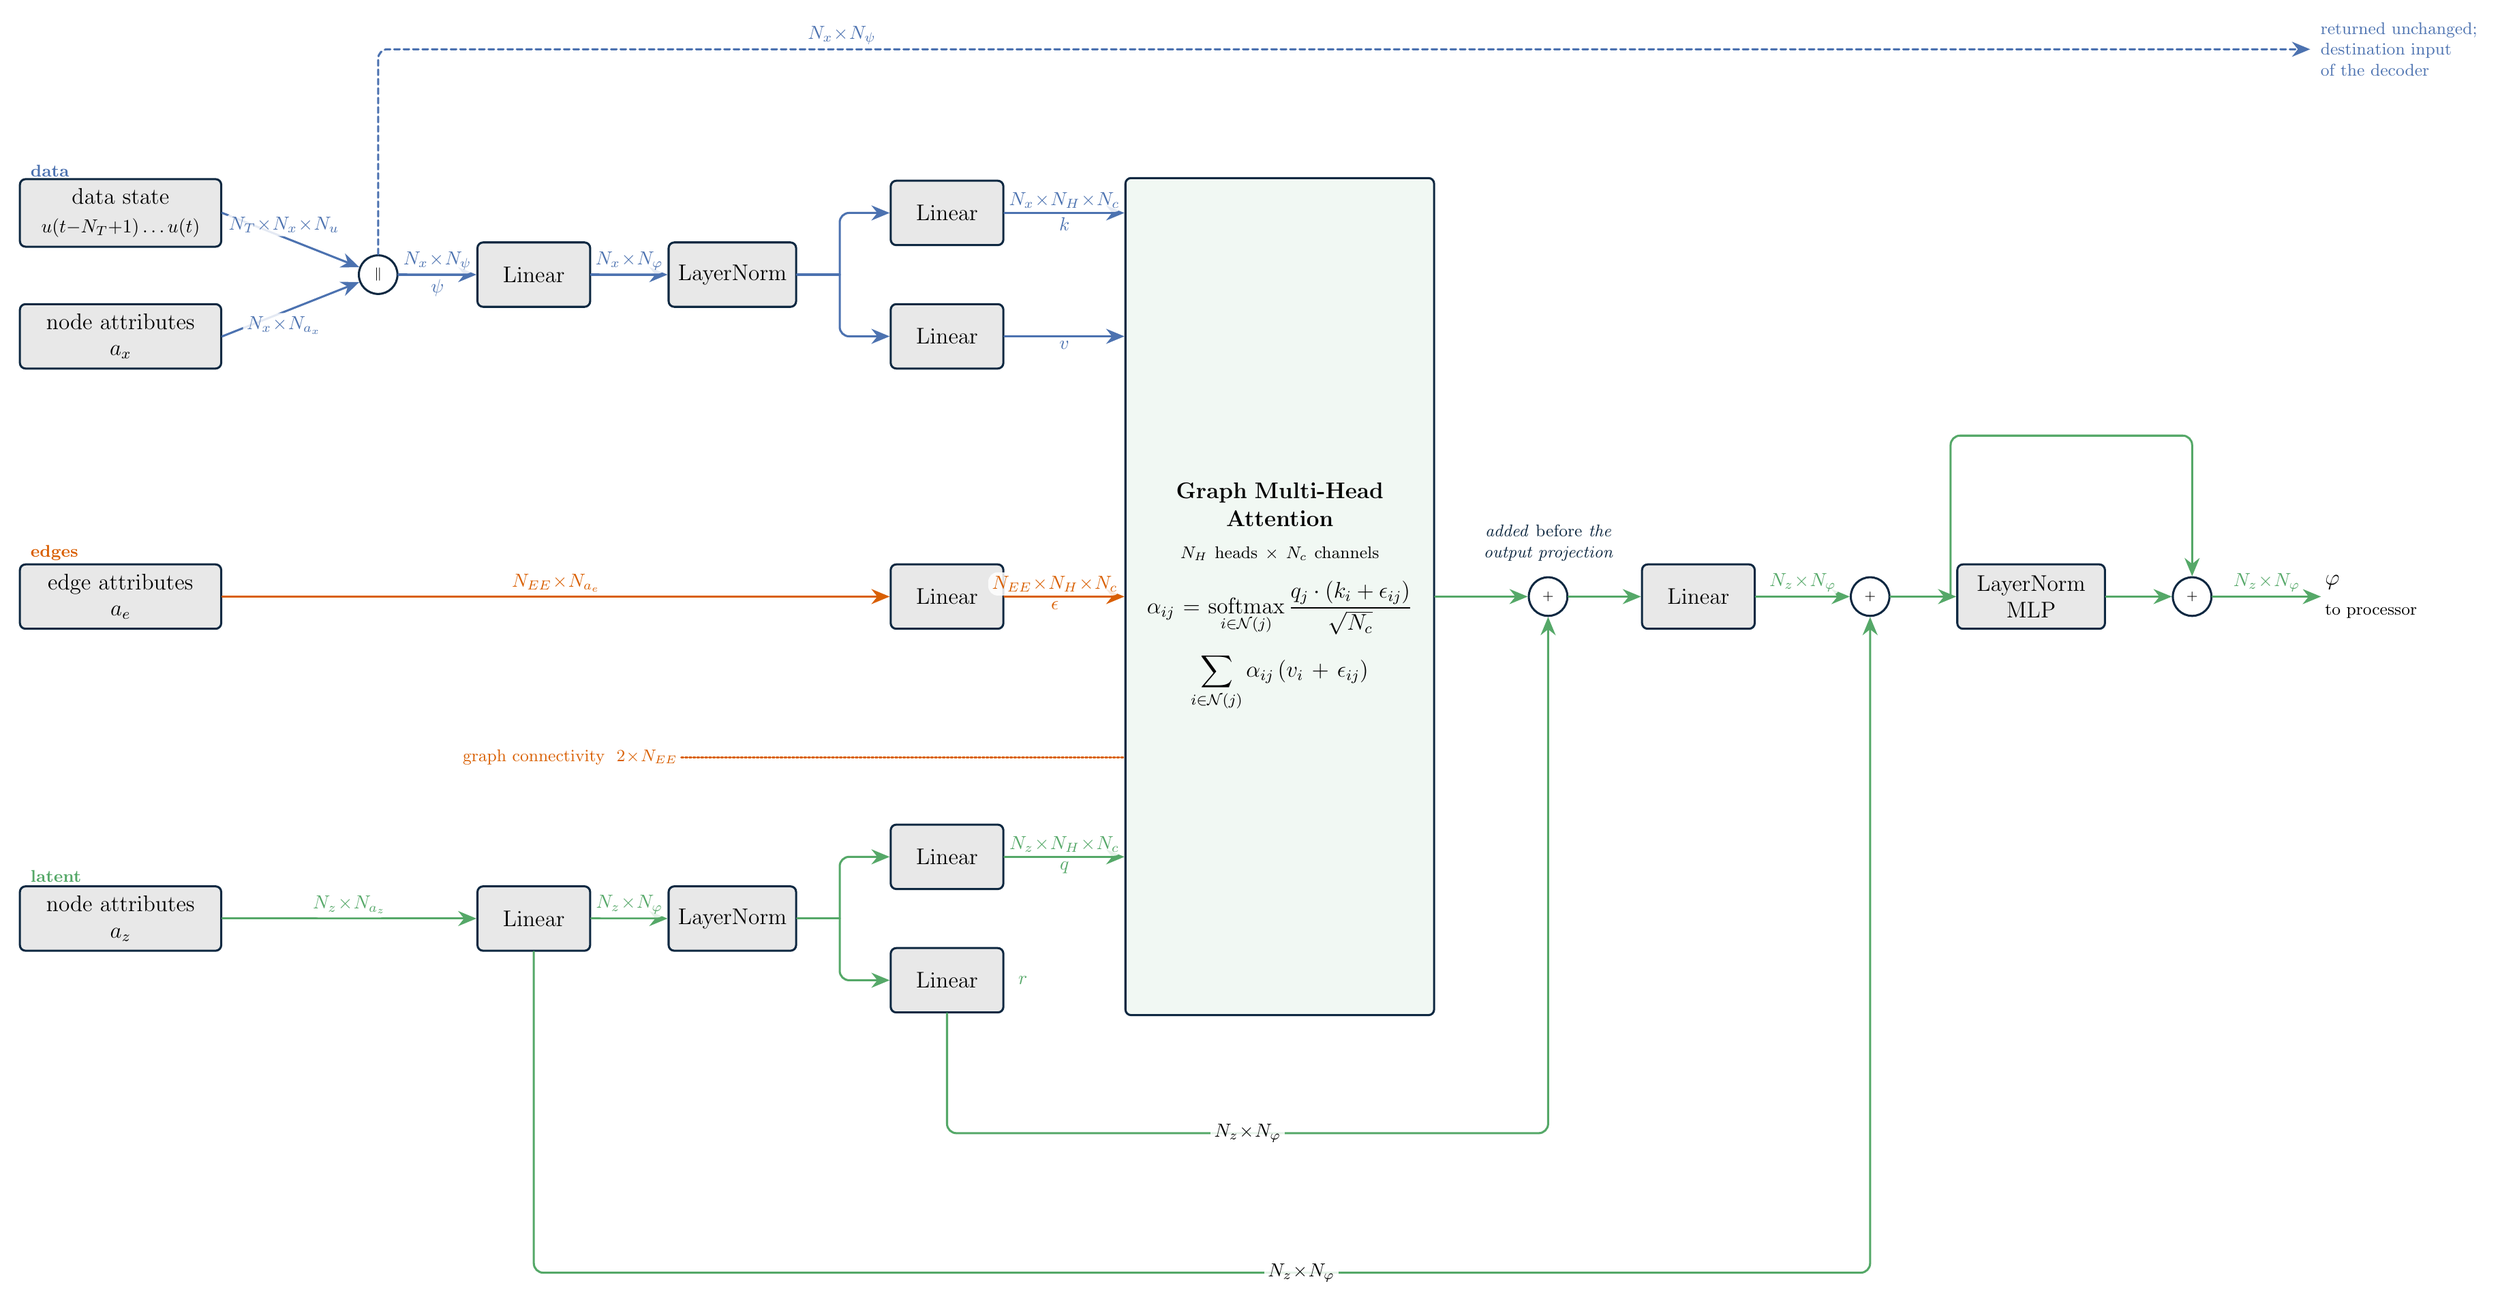
\begin{tikzpicture}[
  x=1cm, y=1cm, font=\large,
  blk/.style     = {rounded corners=3pt, draw=trapline, fill=trapfill,
                    line width=1.1pt, align=center, inner sep=5pt,
                    minimum height=1.2cm, minimum width=2.1cm},
  attnblk/.style = {blk, fill=attnfill},
  sum/.style     = {circle, draw=trapline, fill=white, line width=1.1pt,
                    inner sep=0pt, minimum size=0.72cm},
  term/.style    = {align=center, inner sep=2pt},
  wire/.style    = {-{Stealth[length=3.4mm,width=2.8mm]}, line width=1.1pt,
                    line cap=round, rounded corners=5pt},
  plain/.style   = {line width=1.1pt, line cap=round, rounded corners=5pt},
  shp/.style     = {font=\normalsize, inner sep=2pt, fill=white,
                    fill opacity=0.85, text opacity=1},
  tag/.style     = {font=\normalsize\itshape, inner sep=2pt},
  lane/.style    = {font=\small\bfseries, anchor=south west},
]

% =========================== lane labels ====================================
% anchored on the left edge of the input boxes so nothing overhangs the
% bounding box (the standalone crop would clip it)
\node[lane, text=dataclr]   at ({\colA-1.8}, {\rowdata+\stack+0.55}) {data};
\node[lane, text=edgeclr]   at ({\colA-1.8}, {\rowedge+0.55})        {edges};
\node[lane, text=latentclr] at ({\colA-1.8}, {\rowlat+0.55})         {latent};

% =========================== DATA LANE ======================================
\node[blk, text width=3.4cm] (uin)  at (\colA, {\rowdata+\stack})
  {data state\\[1pt]{\normalsize$\datavec(t{-}\NT{+}1)\dots\datavec(t)$}};
\node[blk, text width=3.4cm] (axin) at (\colA, {\rowdata-\stack})
  {node attributes\\$\attrx$};
\node[sum] (cat)  at (\colcat, \rowdata) {\scriptsize$\|$};
\node[blk] (embx) at (\colB, \rowdata) {Linear};
\node[blk] (lnx)  at (\colC, \rowdata) {LayerNorm};
\node[blk] (link) at (\colD, {\rowdata+1.15}) {Linear};
\node[blk] (linv) at (\colD, {\rowdata-1.15}) {Linear};
\coordinate (xsplit) at (\colsplit, \rowdata);

\draw[wire, dataclr] (uin.east)  -- node[shp, above, pos=0.45]
  {\shapethree{\NT}{\Nx}{\Nu}} (cat);
\draw[wire, dataclr] (axin.east) -- node[shp, below, pos=0.45]
  {\shapetwo{\Nx}{\Nax}} (cat);
\draw[wire, dataclr] (cat) -- node[shp, above] {\shapetwo{\Nx}{\Npsi}}
                             node[tag, below, text=dataclr] {$\inputvec$} (embx);
\draw[wire, dataclr] (embx) -- node[shp, above] {\shapetwo{\Nx}{\Nphi}} (lnx);
\draw[plain, dataclr] (lnx.east) -- (xsplit);
\draw[wire, dataclr] (xsplit) |- (link.west);
\draw[wire, dataclr] (xsplit) |- (linv.west);

% the mapper returns its source input untouched; it is the decoder's dst input
\draw[wire, dataclr, densely dashed] (cat.north) |- (\colK, \rowbypass)
  node[shp, above, pos=0.62] {\shapetwo{\Nx}{\Npsi}}
  node[term, anchor=west, xshift=3pt, align=left, font=\small]
  {returned unchanged;\\destination input\\of the decoder};

% =========================== EDGE LANE ======================================
\node[blk, text width=3.4cm] (aein) at (\colA, \rowedge)
  {edge attributes\\$\attre$};
\node[blk] (line) at (\colD, \rowedge) {Linear};
\node[term, anchor=west, align=left, font=\small, text=edgeclr,
      fill=white, inner sep=2pt] (conn)
  at ({\colB-1.4}, \rowconn) {graph connectivity\ \ $2\!\times\!\NEE$};

\draw[wire, edgeclr] (aein) -- node[shp, above] {\shapetwo{\NEE}{\Nae}} (line);

% =========================== LATENT LANE ====================================
\node[blk, text width=3.4cm] (azin) at (\colA, \rowlat)
  {node attributes\\$\attrz$};
\node[blk] (embz) at (\colB, \rowlat) {Linear};
\node[blk] (lnz)  at (\colC, \rowlat) {LayerNorm};
\node[blk] (linq) at (\colD, {\rowlat+1.15}) {Linear};
\node[blk] (lins) at (\colD, {\rowlat-1.15}) {Linear};
\coordinate (zsplit) at (\colsplit, \rowlat);

\draw[wire, latentclr] (azin) -- node[shp, above] {\shapetwo{\Nz}{\Naz}} (embz);
\draw[wire, latentclr] (embz) -- node[shp, above] {\shapetwo{\Nz}{\Nphi}} (lnz);
\draw[plain, latentclr] (lnz.east) -- (zsplit);
\draw[wire, latentclr] (zsplit) |- (linq.west);
\draw[wire, latentclr] (zsplit) |- (lins.west);

% =========================== ATTENTION ======================================
\node[attnblk, minimum height=15.6cm, text width=5.4cm] (attn) at (\colE, \rowedge)
  {\textbf{Graph Multi-Head}\\[1pt]\textbf{Attention}\\[3pt]
   {\small $\NH$ heads $\times$ $\Nc$ channels}\\[10pt]
   {\large$\displaystyle
      \attn_{ij}=\operatorname*{softmax}_{i\in\nbhd(j)}
      \frac{\query_j\cdot(\keyv_i+\edgeemb_{ij})}{\sqrt{\Nc}}$}\\[9pt]
   {\large$\displaystyle
      \sum_{i\in\nbhd(j)}\attn_{ij}\,(\valuev_i+\edgeemb_{ij})$}};

\draw[wire, dataclr] (link.east) -- node[shp, above]
  {\shapethree{\Nx}{\NH}{\Nc}} node[tag, below, text=dataclr] {$\keyv$}
  (link.east -| attn.west);
\draw[wire, dataclr] (linv.east) -- node[tag, below, text=dataclr] {$\valuev$}
  (linv.east -| attn.west);
\draw[wire, edgeclr] (line.east) -- node[shp, above, pos=0.42]
  {\shapethree{\NEE}{\NH}{\Nc}} node[tag, below, pos=0.42, text=edgeclr] {$\edgeemb$}
  (line.east -| attn.west);
\draw[wire, latentclr] (linq.east) -- node[shp, above]
  {\shapethree{\Nz}{\NH}{\Nc}} node[tag, below, text=latentclr] {$\query$}
  (linq.east -| attn.west);
\draw[plain, edgeclr, densely dotted] (conn.east) -- (conn.east -| attn.west);

% =========================== POST-ATTENTION CHAIN ===========================
\node[sum] (res1) at (\colF, \rowedge) {\scriptsize$+$};
\node[blk] (proj) at (\colG, \rowedge) {Linear};
\node[sum] (res2) at (\colH, \rowedge) {\scriptsize$+$};
\node[blk, text width=2.4cm] (ff) at (\colI, \rowedge)
  {LayerNorm\\MLP};
\node[sum] (res3) at (\colJ, \rowedge) {\scriptsize$+$};
\node[term, anchor=west, align=left] (out) at ({\colK+0.2}, \rowedge)
  {$\latentvec$\\[2pt]{\small to processor}};

\draw[wire, latentclr] (attn.east) -- (res1);
\draw[wire, latentclr] (res1) -- (proj);
\node[tag, above=6pt of res1, text=trapline, align=center]
  {\small added \emph{before} the\\[-1pt]\small output projection};
\draw[wire, latentclr] (proj) -- node[shp, above] {\shapetwo{\Nz}{\Nphi}} (res2);
\draw[wire, latentclr] (res2) -- (ff);
\draw[wire, latentclr] (ff) -- (res3);
\draw[wire, latentclr] (res3) -- node[shp, above] {\shapetwo{\Nz}{\Nphi}} (out);


% residual 1 -- the self branch, added in attention space, ahead of the
% output projection (AIAYN draws that projection inside its attention box)
\draw[wire, latentclr] (lins.south) |- ({\colF}, \rowselfskip) -- (res1.south);
\node[shp] at ({(\colD+\colF)/2}, \rowselfskip) {\shapetwo{\Nz}{\Nphi}};
\node[tag, anchor=west, text=latentclr]
  at ({\colD+1.25}, {\rowlat-1.15}) {$\selfv$};

% residual 2 -- pre-norm skip taken from the latent embedding
\draw[wire, latentclr] (embz.south) |- ({\colH}, \rowdstskip) -- (res2.south);
\node[shp] at ({(\colC+\colH)/2}, \rowdstskip) {\shapetwo{\Nz}{\Nphi}};

% residual 3 -- pre-norm skip around the MLP
\draw[wire, latentclr] ({(\colH+\colI)/2}, \rowedge) |- ({\colJ}, \rowffskip)
  -- (res3.north);

\end{tikzpicture}
}
\end{center}
\vspace*{\fill}

{\footnotesize
    \textbf{Encoder.}\;
    \texttt{GraphTransformerForwardMapper} maps the data-space
    state onto the latent mesh.
    Shapes are given for a single batch element and a
    single ensemble member; the batch and ensemble axes are flattened into the node
    axis before the encoder is called.
    Three residual paths act on the latent
    stream and none on the data stream: the source nodes are returned unchanged
    (\texttt{update\_src\_nodes = False}) and are discarded by the caller.
    The embedded edge attributes $\edgeemb$ enter the
    attention twice: into the key, where they steer the weight, and into the value,
    where they steer the payload.
    The softmax runs over the incoming edges of each
    latent node separately and per head --- not over all $\Nx\!\times\!\Nz$ pairs.
    The mapper's chunking
    (\texttt{num\_chunks}) partitions the latent nodes and, because the edge index
    is sorted by destination, is exact --- it is a memory optimisation only and is
    not drawn.
\par}

\clearpage

% ============================== page 2 =====================================
\begin{center}
  \begin{minipage}{0.72\textwidth}
    \section*{Notation}

    Lowercase letters denote variables and functions; integer counts are written
    $N_{\text{quantity}}$.  Values are read directly from the checkpoint by
    \texttt{extract\_dims.py}, so they cannot drift from the trained model.

    \medskip
    \begin{tabular}{@{}llr@{}}
      \toprule
      symbol & meaning & value \\
      \midrule
      \symbolrows
      \bottomrule
    \end{tabular}

    \medskip
    {\footnotesize
    $\|$ denotes concatenation along the feature axis.  The attribute widths
    split as (sin/cos lat-lon) $\|$ (trainable), and the edge attribute width as
    (length, direction) $\|$ (trainable); the trainable parts are
    zero-initialised.  $\NEE$ counts the encoder's data-to-latent edges;
    $N_{DE}$ is reserved for the decoder's.

    \smallskip
    Each latent node draws on a small local patch of the data mesh rather than
    on all of it: in this graph $\nbhd(\coordz_j)$ holds between \valdegmin\ and
    \valdegmax\ data nodes, \valdegmean\ on average.  It is empty for
    \valdegzero\ of the \valNz\ latent nodes, which by design receive no data
    and carry only their attributes and the skip connection into the processor.
    \par}
  \end{minipage}
\end{center}

\clearpage

% ============================== page 3 =====================================
% Points where this encoder departs from GraphCast-style message passing, from a
% plain GNN, or from a standard transformer.  Each is grounded in the source; the
% numbers come from dims.tex so they track the checkpoint.
\section*{Notes}

Where this encoder departs from GraphCast-style message passing, from a plain GNN,
or from a standard transformer --- and what each departure might be costing.  Line
references are to \texttt{anemoi-core}.

\begin{multicols}{2}
\small\sloppy  % narrow columns; prefer loose lines over overfull ones
\begin{itemize}[leftmargin=1.1em]\setlength{\itemsep}{0.5em}

    \item \textbf{Aggregation is degree-normalised; GraphCast's is not.}
      The softmax makes $\sum_{i\in\nbhd(\coordz_j)}\attn_{ij}=1$, so a latent
      node with one neighbour and one with fifteen both emit a unit-weight
      average.  GraphCast instead \emph{sums} MLP messages over incoming edges,
      so its aggregate grows with degree.  For a data-assimilation-like problem
      the observation density \emph{is} much of the signal, and here the
      attention output carries no magnitude cue for how well observed a patch
      is.  The \texttt{obs\_count} channels ride in $\inputvec$ and so reach the
      values, but that is an indirect route --- worth checking whether the model
      actually exploits it.

    \item \textbf{Edge features are never updated.}
      GraphCast is an interaction network: each message-passing step rebuilds
      edge features from (sender, receiver, edge).  Here $\attre$ passes through
      one Linear into the keys and values and is returned unchanged
      (\texttt{block.py:1029}), then discarded by the mapper
      (\texttt{mapper.py:321}).  Edge geometry is a fixed bias, never a state, so
      it cannot be modulated by the flow it is carrying.

    \item \textbf{The edge embedding enters both the key and the value.}
      \texttt{conv.py:140} and \texttt{:147}, the same tensor twice.  Inherited
      from PyG's \texttt{TransformerConv} rather than invented here, but it is
      distinct both from GraphCast (which concatenates edge features into an MLP)
      and from a plain transformer (no edge features at all).  One
      \texttt{lin\_edge} is trained to do two different jobs: shift the logit and
      shift the payload.

    \item \textbf{There is no self-loop in the softmax.}
      In standard self-attention a token sits inside its own softmax, so
      ``attend to myself'' competes with ``attend to my neighbours'' on a
      normalised scale.  Here the node's own state re-enters outside the softmax,
      through $\selfv$.  The balance between own-state and neighbour-evidence is
      therefore set by the learned magnitude of \texttt{lin\_self} and is
      unbounded --- nothing stops it from swamping, or being swamped by, the
      aggregated data.

    \item \textbf{$\selfv$ is added \emph{before} the output projection, so it is
      not a skip connection.}
      \texttt{block.py:1017} computes \texttt{projection(out + x\_r)}; the
      genuine pre-norm residual is the separate add on the next line.  A standard
      transformer adds its residual \emph{after} $W^O$.  Here the self branch is
      mixed by the projection along with the attention output.

    \item \textbf{The decoder's skip carries raw, un-embedded $\inputvec$.}
      The mapper returns \texttt{x[0]} untouched (\texttt{mapper.py:597}), and
      the decoder re-embeds it with its own Linear.  So
      \texttt{emb\_nodes\_src} serves the keys and values only and never reaches
      the decoder, and the data-space input is embedded twice by two independent
      matrices.  GraphCast's decoder consumes the \emph{encoded} grid features
      instead.  A candidate ablation.

    \item \textbf{\valgraphpct\% of the model's parameters are pinned to
      specific nodes and edges.}
      The trainable node and edge attributes total \valgraphparams\
      (\valnodeparams\ node $+$ \valedgeparams\ edge) against \valencparams\ in
      the entire encoder module and \valtotalparams\ in the whole model --- so
      there is roughly $1.5\times$ as much free parameter attached to \emph{this
      graph} as there is learned weight in the encoder that uses it.  They are
      zero-initialised, they can memorise per-location behaviour, and none of it
      transfers to a different graph or resolution.  Worth inspecting their
      magnitude after training, and worth suspecting first if the model
      generalises poorly in space.

    \item \textbf{The encoder is a single attention block.}
      \texttt{self.proc} is one \texttt{Graph\-Transformer\-Mapper\-Block}, not a stack
      (\texttt{mapper.py:222}); all depth lives in the processor.  GraphCast's
      encoder is likewise a single message-passing step, so this matches --- but
      combined with the one-hop neighbourhood it means the entire path from data
      to latent is one local gather.

    \item \textbf{Multi-dataset latents are summed, not gated.}
      Every dataset contributes additively with no learned weighting between
      them, and each carries its own copy of the latent-attribute residual
      (\texttt{encoder\_\-processor\_\-decoder.py:273}).  Relevant before adding a
      second dataset whose observation density differs sharply from this one's.

\end{itemize}
\end{multicols}

\end{document}
